%%%%%%%%%%%%%%%%%%%%%%%%%%%%%%%%%%%%%%%%%%%%%%%%%%%%%%%%%%%%%%%%%%%%%%%%%%%
%
%		Relazione del progetto di Design Patterns
%
%				    Nicola Corti - 2014
%
%%%%%%%%%%%%%%%%%%%%%%%%%%%%%%%%%%%%%%%%%%%%%%%%%%%%%%%%%%%%%%%%%%%%%%%%%%%
\documentclass[a4paper,12pt]{article} 
\usepackage{graphicx}
\usepackage{vmargin}
\usepackage[italian]{babel} 
\usepackage[utf8x]{inputenc}
\usepackage{listings}
\usepackage{url}
\usepackage{pdflscape}
\usepackage{tabularx}
\usepackage{hyperref}
\usepackage{amsfonts}
\usepackage[usenames,dvipsnames,svgnames,table]{xcolor}
\usepackage{pbox}

\usepackage{caption}
\usepackage{subcaption}

\setlength{\parskip}{8pt}

% Padding tabella
\renewcommand{\arraystretch}{2.5}

%\usepackage{chngcntr}
%\counterwithin{equation}{subsection}

\renewcommand\lstlistingname{Codice}
\addto\captionsitalian{\renewcommand\figurename{Immagine}}

%\setpapersize{A4}
%\setmarginsrb{15mm}{10mm}{15mm}{10mm}%
%             {0mm}{10mm}{0mm}{10mm}


\definecolor{LightLightGray}{RGB}{241,241,241}

\lstset{
basicstyle=\scriptsize\ttfamily,
keywordstyle=\color{MidnightBlue}\bfseries,
identifierstyle=\color{Black},
commentstyle=\color{Green}\itshape,
stringstyle=\color{Red}\ttfamily,
showstringspaces=false,
%numbers=left, numberstyle=\tiny,
%stepnumber=1, numbersep=10pt,
tabsize=4,
framexleftmargin=5mm, rulesepcolor=\color{LightLightGray},
frame=tb,
backgroundcolor=\color{LightLightGray},
%language={Java},
%mathescape=true,
%fontadjust=true,
breaklines=true,breakatwhitespace=true,breakautoindent
}

\title{\emph{StarCastle} - Esempio di applicazione dei design pattern nella modellazione di un videogioco}
\author{Nicola Corti - 454413 \\Corso di Laurea Magistrale in Informatica \\ Universit\`a degli studi di Pisa \\ \\ 
\includegraphics[width=2cm]{unipi.pdf}}
\date{10 Novembre 2014}

 
\begin{document}
\maketitle

\begin{abstract}
Questa relazione ha lo scopo di illustrare come i design pattern possono essere utilizzati nella modellazione di un software complesso, quale pu\`o essere un videogioco. Gli aspetti da tenere in considerazione sono svariati, dal mantenimento di uno stato consistente, alla gestione degli eventi, delle collisioni, etc\dots{}

Il codice sorgente allegato \`e da considerarsi parte integrante di questa relazione, al fine di permettere una comprensione pi\`u organica di tutti gli aspetti di design ed implementativi.
\end{abstract}
\newpage

\tableofcontents
\newpage

\section*{Introduzione}
\label{sec:introduzione}

I videogiochi rappresentano forse la categoria di software pi\`u complessi da realizzare, coinvolgendo in un unico progetto svariati aspetti dell'informatica (si pensi al networking, all'intelligenza artificiale o alla gestione dei database).

La realizzazione di un videogioco, se non supportata da un'accurata fase di analisi e di progettazione, pu\`o risultare veramente complessa o addirittura impossibile. Tralasciare la fase di progettazione di un videogioco potrebbe portare a notevoli perdite di tempo o addirittura al fallimento del progetto stesso.

Per questo motivo risulta fondamentale analizzare sotto ogni aspetto il videogioco che si intende realizzare, e progettare ogni classe/interfaccia con la massima accuratezza. In questa fase dello sviluppo i \emph{design pattern} possono essere un strumento valido per risolvere alcune delle problematiche pi\`u comuni e ricorrenti nel campo dello sviluppo di videogiochi.

In particolare in questa relazione mostreremo come i \emph{design pattern} possono essere di supporto nella progettazione del videogioco \emph{StarCastle}\footnote{\url{http://en.wikipedia.org/wiki/Star_Castle}}, un videogioco vettoriale del 1980 prodotto da Cinematronics\footnote{\`E possibile testare una demo online del gioco all'indirizzo seguente \\ \url{http://www.download-free-games.com/online/game/star_castle/}}.

In \emph{StarCastle} il giocatore si trover\`a a comandare un'astronave spaziale, e dovr\`a attaccare un cannone posto al centro dello schermo (vedi immagine \ref{img:screen}). Il cannone \`e protetto da 3 annelli formate da barre di energie ed \`e in grado di attaccare il giocatore tramite mine (che inseguiranno l'astronave del giocatore) e sfere al plasma (che verranno sparate direttamente dal cannone verso l'astronave). 

\begin{figure}
\centering
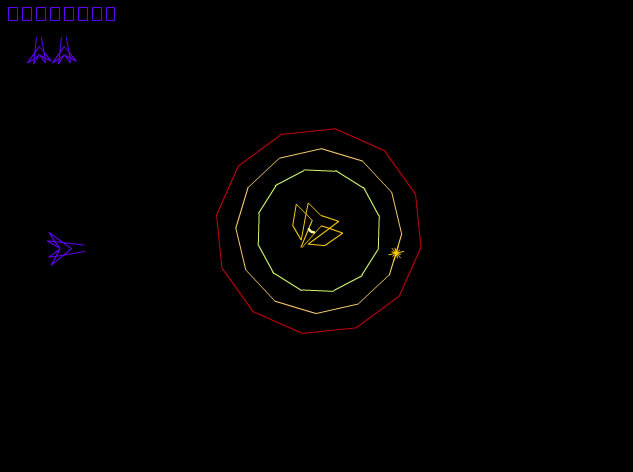
\includegraphics[width=6cm]{screen.jpg}
\caption{Una schermata di gioco di \emph{StarCastle}}
\label{img:screen}
\end{figure}

Tralasciamo una discussione pi\`u dettagliata di tutte le meccaniche di gioco, in quanto verranno analizzate singolarmente nelle varie sezioni seguenti.

Preferiamo piuttosto soffermarci su un pattern che ha guidato la fase di progettazione di tutto il software e che permea tutti gli aspetti che verranno analizzati nelle sezioni seguenti, il \emph{Model-View-Controller}.

\subsection*{Il pattern \emph{Model-View-Controller}}

Il \emph{Model-View-Controller} \`e un pattern architetturale che ha come scopo principale quello di mettere il focus sulla separazione fra la rappresentazione dei dati e la loro rappresentazione.

I componenti che interagiscono nel pattern \emph{Model-View-Controller}, come suggerisce il nome, sono 3 (vedi immagine \ref{img:mvc}):

\begin{description}
\item[\textsf{Model}] Mantiene la rappresentazione dei dati e si occupa della \emph{business logic},
\item[\textsf{View}] Interagisce con il \textsf{Model} e offre all'utente una sua rappresentazione visuale,
\item[\textsf{Controller}] Raccoglie l'input dell'utente e modifica il \textsf{Model} di conseguenza.
\end{description}

\begin{figure}[h]
\centering
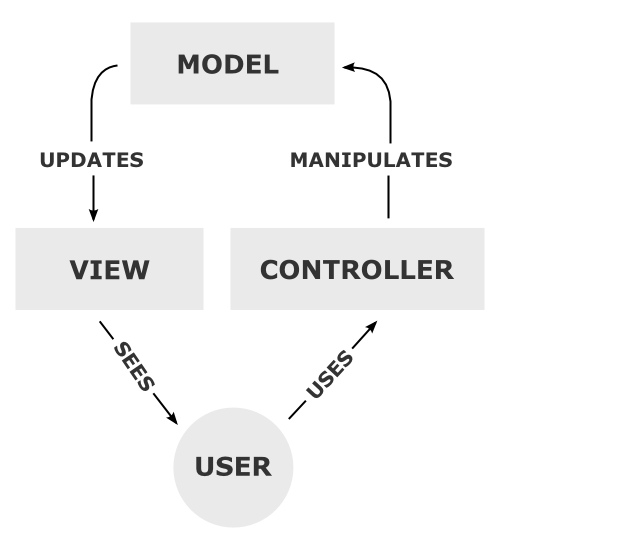
\includegraphics[width=5cm]{mvc.png}
\caption{Diagramma del pattern \emph{Model-View-Controller}}
\label{img:mvc}
\end{figure}

In particolare in \emph{StarCastle} sono stati i componenti del \emph{Model-View-Controller} sono stati istanziati come segue:

\begin{description}
\item[\textsf{Model}] Rappresenta lo stato di tutte le entit\`a di gioco, mantenendone stato attuale, posizione, velocit\`a ed eventuali interazioni con altre entit\`a di gioco
\item[\textsf{View}] Rappresenta il contesto grafico sul quale verranno disegnate tutte le primitive grafiche per rappresentare i vari componenti del gioco, secondo le policy grafiche previste dal sistema
\item[\textsf{Controller}] Rappresenta il meccanismo che si occupa di raccogliere gli input dell'utente, e di convertirli in comandi di giochi, che verranno elaborati al fine di far evolvere le entit\`a in gioco (nella fattispecie quindi muovere o far sparare una navicella).
\end{description}

\section{Modellazione della realt\`a}
\label{sec:stato}

Il primo passo effettuato nella fase di progettazione di dettaglio consiste nell'individuare quali saranno le classi che andranno a rappresentare la nostra realt\`a.

Analizzando il nostro caso ci rendiamo subito conto che:
\begin{itemize}
\item Le entit\`a da modellare sono fondamentalmente 5: l'astronave, il cannone, le mine, i missili e le barre di energia.
\item Esse condividono alcuni attributi comuni, quali ad esempio la posizione.
\item Esse condividono dei comportamenti comuni, quali ad esempio la necessit\`a di modificare la propria posizione.
\item Le entit\`a necessitano di mantenere uno stato comune, che muta quando avviene una collisione fra due entit\`a distinte.
\item Alcune entit\`a (cannone e mine) hanno la necessit\`a di essere notificate quando un utente interagisce con il gioco, al fine di poter decidere quale navicella spaziale seguire.
\end{itemize}

Per questi motivi si \`e deciso di progettare una gerarchia di classi che ha come padre la classe astratta \textsf{GameEntity} e di utilizzare i seguenti pattern:
\begin{description}
\item[\emph{State}] Per modellare gli stati delle entit\`a in gioco e le loro transizioni di stato,
\item[\emph{Factory method}] Per delegare la creazione dello stato iniziale alle sottoclassi di \textsf{GameEntity},
\item[\emph{Observer}] Per modellare il meccanismo di notifica di interazione del giocatore alle mine e al cannone.
\end{description}

La gerarchia di classi \`e rappresentata nell'immagine \ref{img:GameEntity}\footnote{Si noti che in questo e nei prossimi diagrammi UML non sono rappresentati tutti gli attrubuti e i metodi della classe, ma solamente quelli significati nel contesto in cui vengono trattati, al fine di non appesantire il diagramma}.

\begin{figure}[ht]
\centering
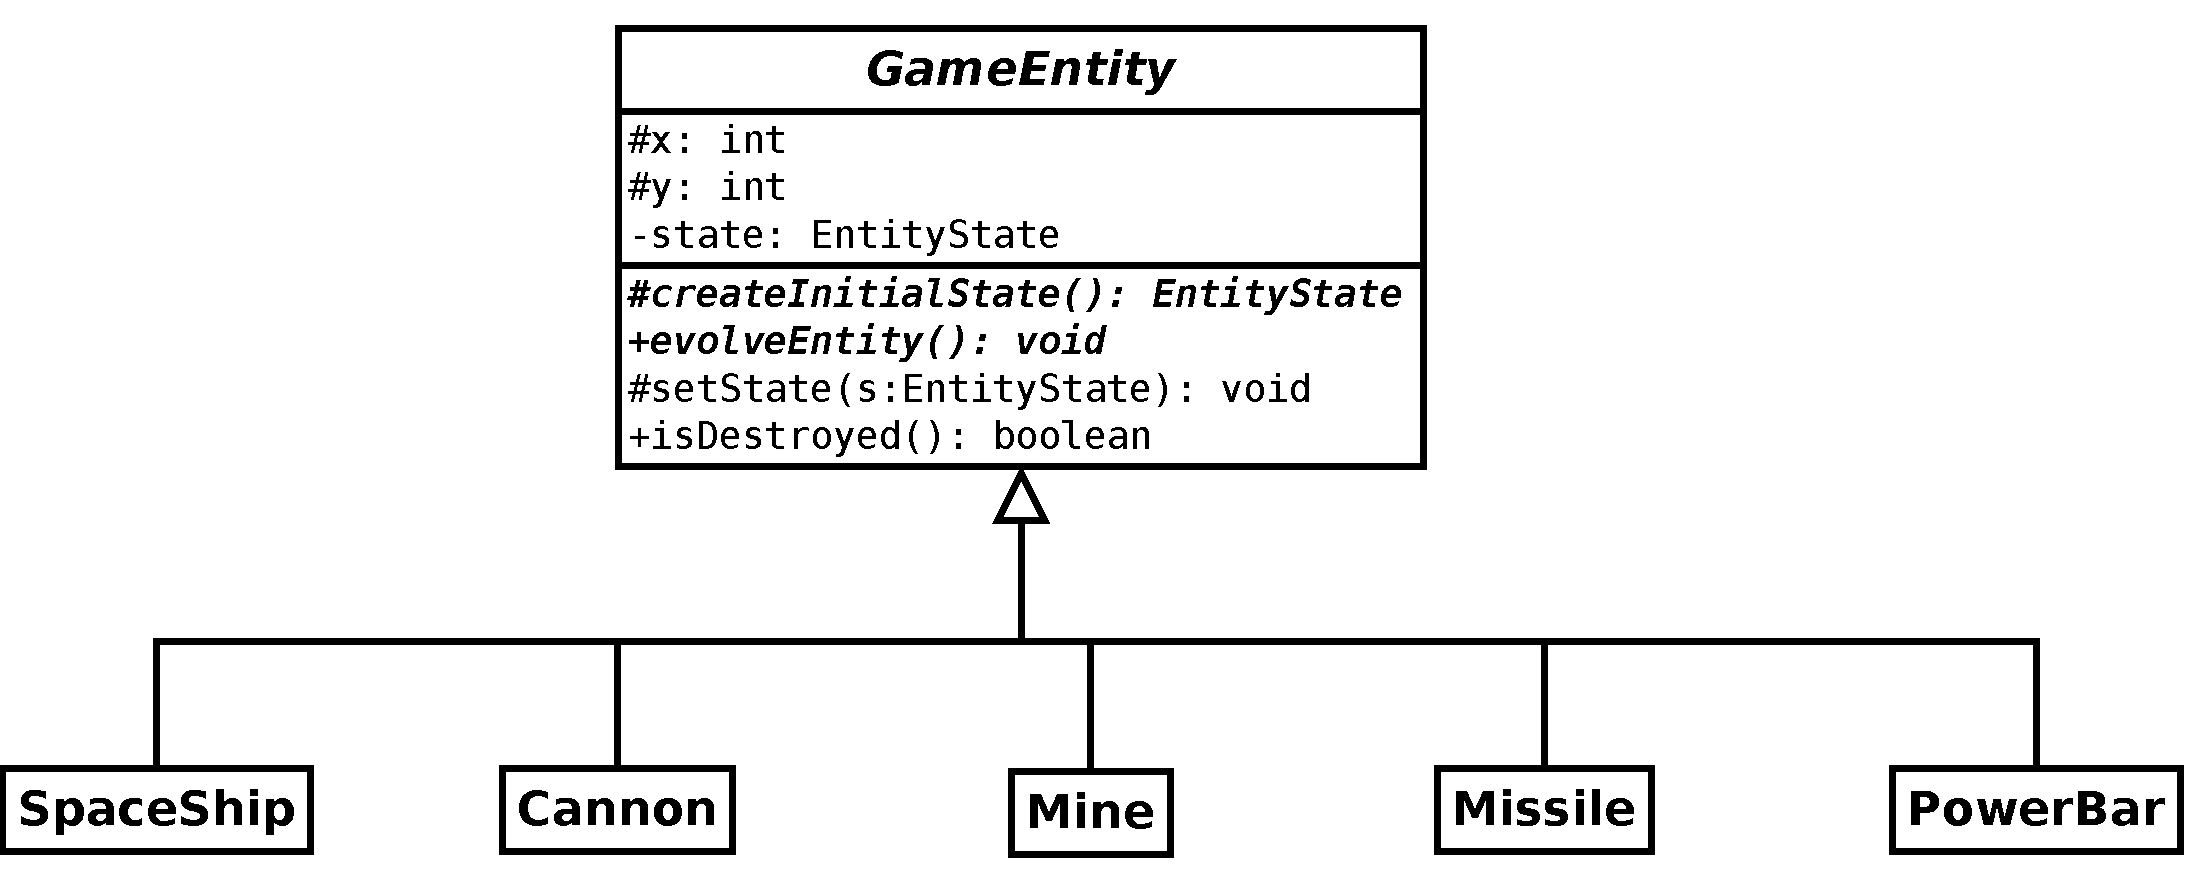
\includegraphics[width=15cm]{GameEntity.pdf}
\caption{Diagramma UML della classe \textsf{GameEntity}}
\label{img:GameEntity}
\end{figure}

Poniamo attenzione al metodo \textsf{evolveEntity}, esso rappresenta il metodo fondamentale per definire come l'entit\`a si evolve nel tempo. \`E un metodo astratto e deve essere implementato da ogni sottoclasse definendo il proprio comportamento (si pensi ad esempio al cannone che ruota, all'astronave che decelera linearmente o ai missili che procedono il linea retta con velocit\`a costante).

Gli altri metodi di \textsf{GameEntity} verranno trattati nel dettagli nelle sezioni seguenti.

\subsection{Utilizzo dal pattern \emph{State}}
\label{sec:state}

Al fine di modellare al meglio la necessit\`a di mantenere uno stato e di evolverlo da parte delle \textsf{GameEntity} si \`e utilizzato il pattern \emph{State}: \`e stata definita la classe astratta \textsf{EntityState} che rappresenta un generico stato di un'entit\`a.

Ogni classe provveder\`a a realizzare le sottoclassi di \textsf{EntityState} e a fornire l'implementazione dei metodi astratti della classe.

\begin{figure}[h]
\centering
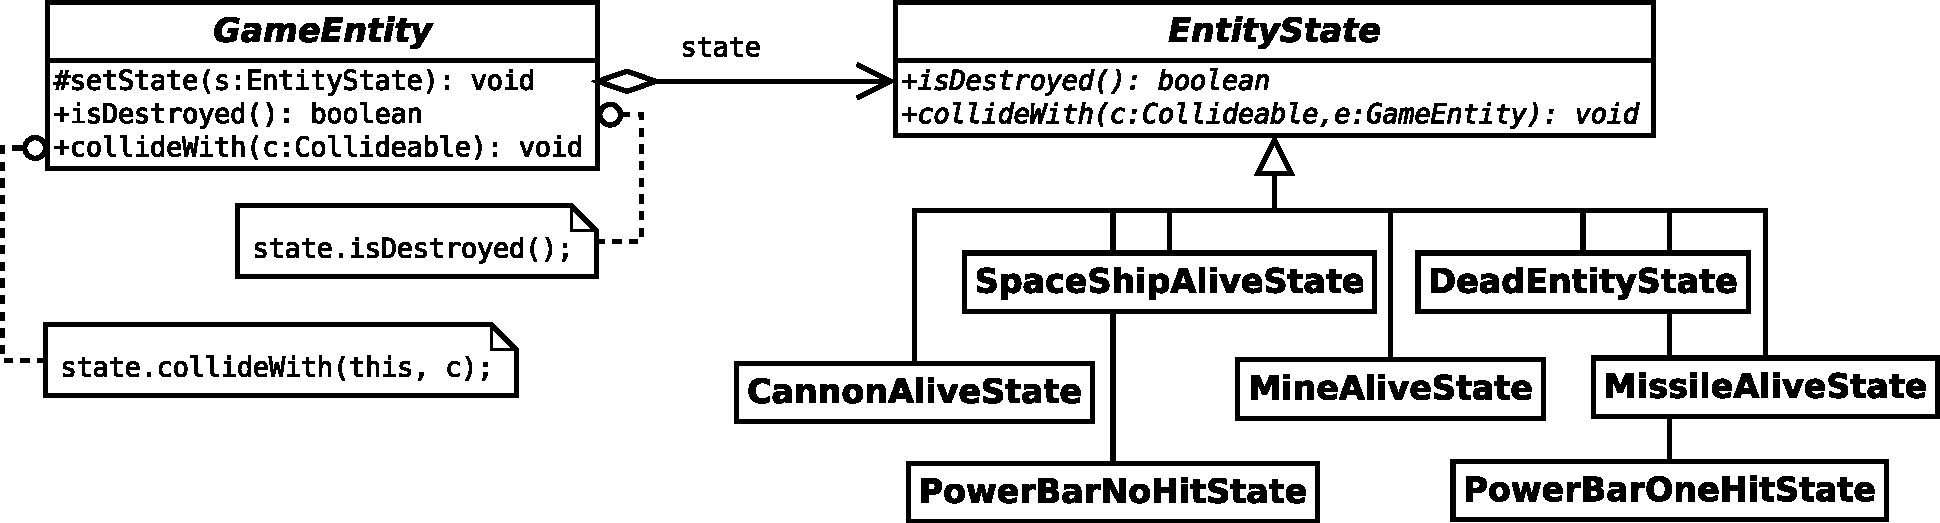
\includegraphics[width=15cm]{State.pdf}
\caption{Diagramma UML del pattern \emph{State}}
\label{img:State}
\end{figure}

Nel diagramma in figura \ref{img:State} si nota che la classe \textsf{EntityState} contiene i metodi: \textsf{isDestroyed} per verificare se l'astronave si trova in uno stato in cui \`e stata distrutta, e \textsf{collideWith} per gestire la collisione fra l'entit\`a e un altro oggetto. (Per la gestione delle collisioni si rimanda alla sezione \ref{sec:collisioni}).

Si noti come il metodo \textsf{collideWith} ha due parametri, il primo rappresenta il riferimento al \textsf{GameEntity} stesso, mentre il secondo rappresenta un oggetto con cui si \`e entrati in collisione; il primo parametro \`e necessario in quanto lo stato invocher\`a il metodo \textsf{setState} sul \textsf{GameEntity} al fine di realizzare la transizione verso un nuovo stato.

Utilizzare il pattern \emph{State} comporta la realizzazione di tante piccole classi che rappresentano i singoli stati delle entit\`a, come si pu\`o notare dalle sottoclassi di \textsf{EntityState} presenti nel diagramma. Questo sembrerebbe introdurre complessit\`a nella progettazione, ma porta invece notevoli benefici, permettendo di evitare grossi statement switch e permettendo di semplificare notevolmente la fase di rendering grafico (sezione \ref{sec:graphics}).

Si noti infine che \`e stata realizzata una singola classe \textsf{DeadEntityState} al fine di rappresentare lo stato in cui termina una generica entit\`a che \`e stata distrutta; invece di realizzare svariate classi del tipo \textsf{SpaceShipDeadState}, \textsf{CannonDeadState}, etc\dots{} riducendo cos\`i la replicazione del codice.

\subsection{Utilizzo del pattern \emph{Factory Method}}
\label{sec:factory}

Per la creazione del primo stato in cui nasce una \textsf{GameEntity} si \`e deciso di utilizzare il pattern \emph{Factory Method}: nella classe \textsf{GameEntity} \`e presente il metodo astratto \textsf{createInitialState}, ogni classe deve quindi implementare questo metodo, costruendo quello che \`e l'oggetto che rappresenta il loro stato iniziale. Per cui ad esempio la classe \textsf{SpaceShip} ritorner\`a un nuovo oggetto di tipo \textsf{SpaceShipAliveState}.

Nel diagramma in figura \ref{img:FactoryMethod} riportiamo le classi relative a \textsf{SpaceShip}, i diagrammi per le altre sottoclassi di \textsf{GameEntity} sono pressoch\'e analoghi.

\begin{figure}[h]
\centering
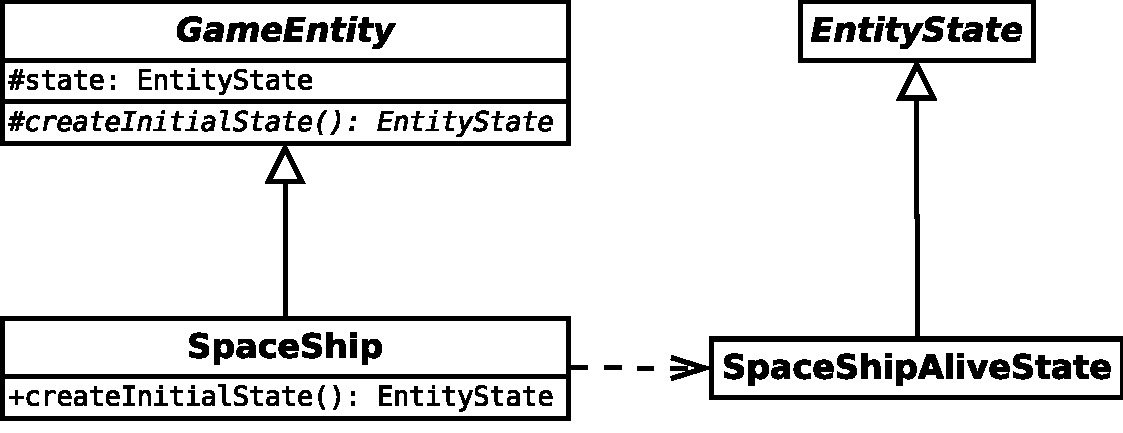
\includegraphics[width=10cm]{FactoryMethod.pdf}
\caption{Diagramma UML del pattern \emph{Factory Method}}
\label{img:FactoryMethod}
\end{figure}

\subsection{Utilizzo del pattern \emph{Observer}}

Per gestire la logica dello spostamento di mine e del cannone, che devono inseguire una delle astronavi in gioco, si \`e deciso di utilizzare il pattern \emph{Observer}.

In particolare, ogni volta che un'astronave riceve un comando di rotazione, accelerazione o di sparo, questa notifica a tutte le mine e al cannone in gioco.

Per implementare il pattern sono stati utilizzati le classi e le interfacce delle Java API: le classi \textsf{Mine} e \textsf{Cannon} implementano l'interfaccia \textsf{java.util.Observer}, fornendo il metodo \textsf{update} che verr\`a invocato ogni volta che ricevono una notifica.

Nell'implementazione attuale le classi \textsf{Mine} e \textsf{Cannon} inseguono l'ultima \textsf{SpaceShip} da cui hanno ricevuto una notifica, ma si potrebbe ampliare la logica prevedendo di seguire l'astronave che ha la distanza minore.

Per quanto riguarda la classe \textsf{SpaceShip} si \`e deciso mantenere un riferimento ad un oggetto di tipo \textsf{DelegatedObservable}, in quanto \textsf{SpaceShip} era gi\`a in una gerarchia di classi. Si noti che la classe \textsf{DelegatedObservable} (sottoclasse di \textsf{java.util.Observable}) \`e una classe necessaria per il meccanismo della delega, in quanto estende la visibilit\`a dei metodi di \textsf{Observable}.

Le classi coinvolte sono riassunte nel diagramma in figura \ref{img:Observer}.

\begin{figure}[ht]
\centering
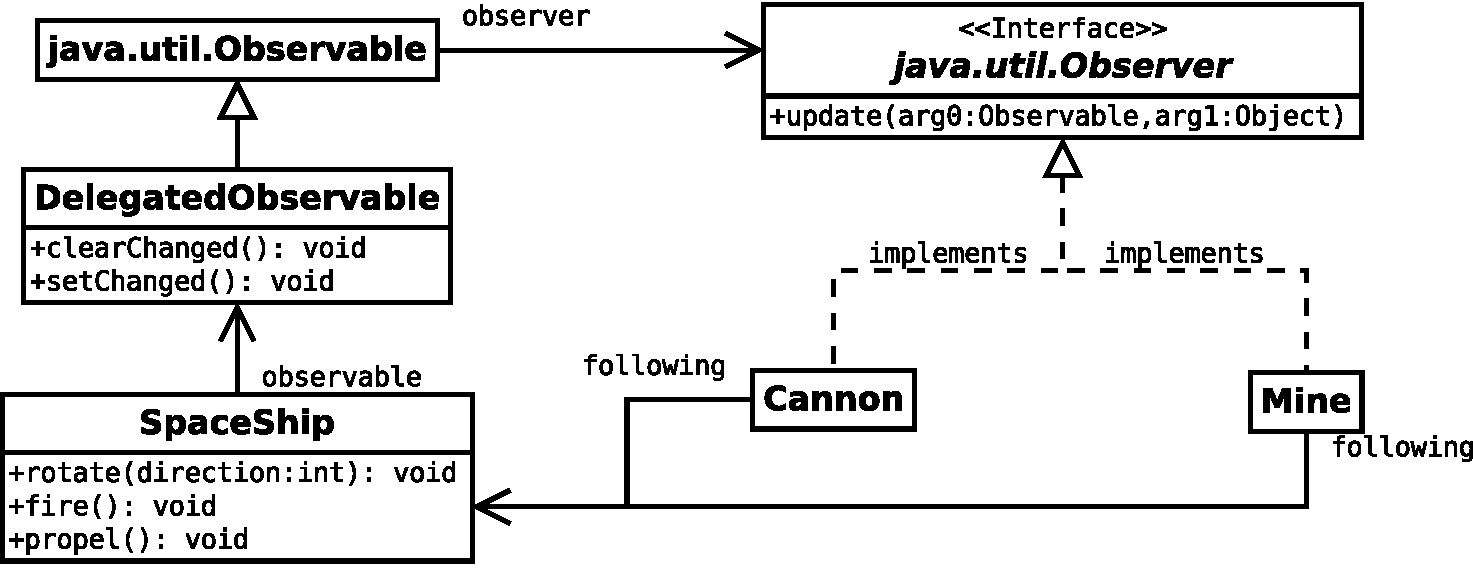
\includegraphics[width=14cm]{Observer.pdf}
\caption{Diagramma UML del pattern \emph{Observer}}
\label{img:Observer}
\end{figure}

\section{Gestione delle collisioni}
\label{sec:collisioni}

Un altro aspetto fondamentale, legato al concetto di stato, \`e quello della gestione delle collisioni. Una gestione delle collisioni mal implementata pu\`o ridurre drasticamente il gameplay di un videogioco, e portare frustrazioni al giocatore con conseguente degrado dell'esperienza utente.

Abbiamo intanto definito un'area circolare, centrata sull'entit\`a e con un determinato raggio, in cui si registrano le collisioni; consideriamo una collisione nel momento in cui queste aree circolari si intersecano in almeno un punto. Quest'area \`e rappresentata dalla classe \textsf{BoundCircle}.

Concettualmente ogni \textsf{GameEntity} dovrebbe controllare ogni altra entit\`a in gioco e verificare se sono presenti delle collisioni, ottenendo il \textsf{BoundCircle} e verificando se si interseca con il proprio.

\subsection{Utilizzo del pattern \emph{Mediator}}

Invece di obbligare ogni \textsf{GameEntity} ad interagire con ogni altra \textsf{GameEntity} presente, abbiamo preferito un approccio pi\`u centralizzato, utilizzando il pattern \emph{Mediator}.

In particolare abbiamo realizzato:
\begin{itemize}
\item L'interfaccia \textsf{Collideable} che deve essere implementata da ogni entit\`a, in particolare \textsf{Collideable} \`e implementata da \textsf{GameEntity} che fornisce direttamente l'implementazione dei due metodi dell'interfaccia:
\begin{itemize}
\item \textsf{getBoundCircle} che ritorna il \textsf{BoundCircle} di una dimensione standard (le sottoclassi faranno l'override di questo metodo se il bound circle \`e differente).
\item \textsf{collideWith} che rappresenta il metodo invocato quando \textsf{GameEntity} entra in collisione con un altro \textsf{Collideable}, implementato invocando il metodo \textsf{collideWith} dello stato attuale (sezione \ref{sec:state}).
\end{itemize}
\item L'interfaccia \textsf{CollisionMediator}, che deve essere implementata dai mediator concreti, con il metodo \textsf{checkCollision} che deve controllare, data una lista di \textsf{Collideable}, se sono presenti collisioni, e notificare i soggetti coinvolti nella collisione 
\item La classe \textsf{CollisionConcreteMediator} che rappresenta un'implementazione concreta dell'interfaccia \textsf{CollisionMediator}.
\end{itemize}

Si noti come questa implementazione del pattern \emph{Mediator} risulta leggermente differente da quella prevista dalla \emph{GoF}: i soggetti \emph{Colleague} previsti dal \emph{GoF} dovrebbero mantenere il riferimento al \emph{Mediator}, mentre nel nostro caso non abbiamo previsto che i \textsf{GameEntity} potessero interagire direttamente con il \textsf{CollisionMediator}, ma che sia il \textsf{CollisionMediator} a richiedere le informazioni per computare le collisioni alle singole \textsf{GameEntity}.

Le classi coinvolte nella gestione delle collisioni sono presentate nel diagramma in figura \ref{img:Mediator}.

\begin{figure}[h]
\centering
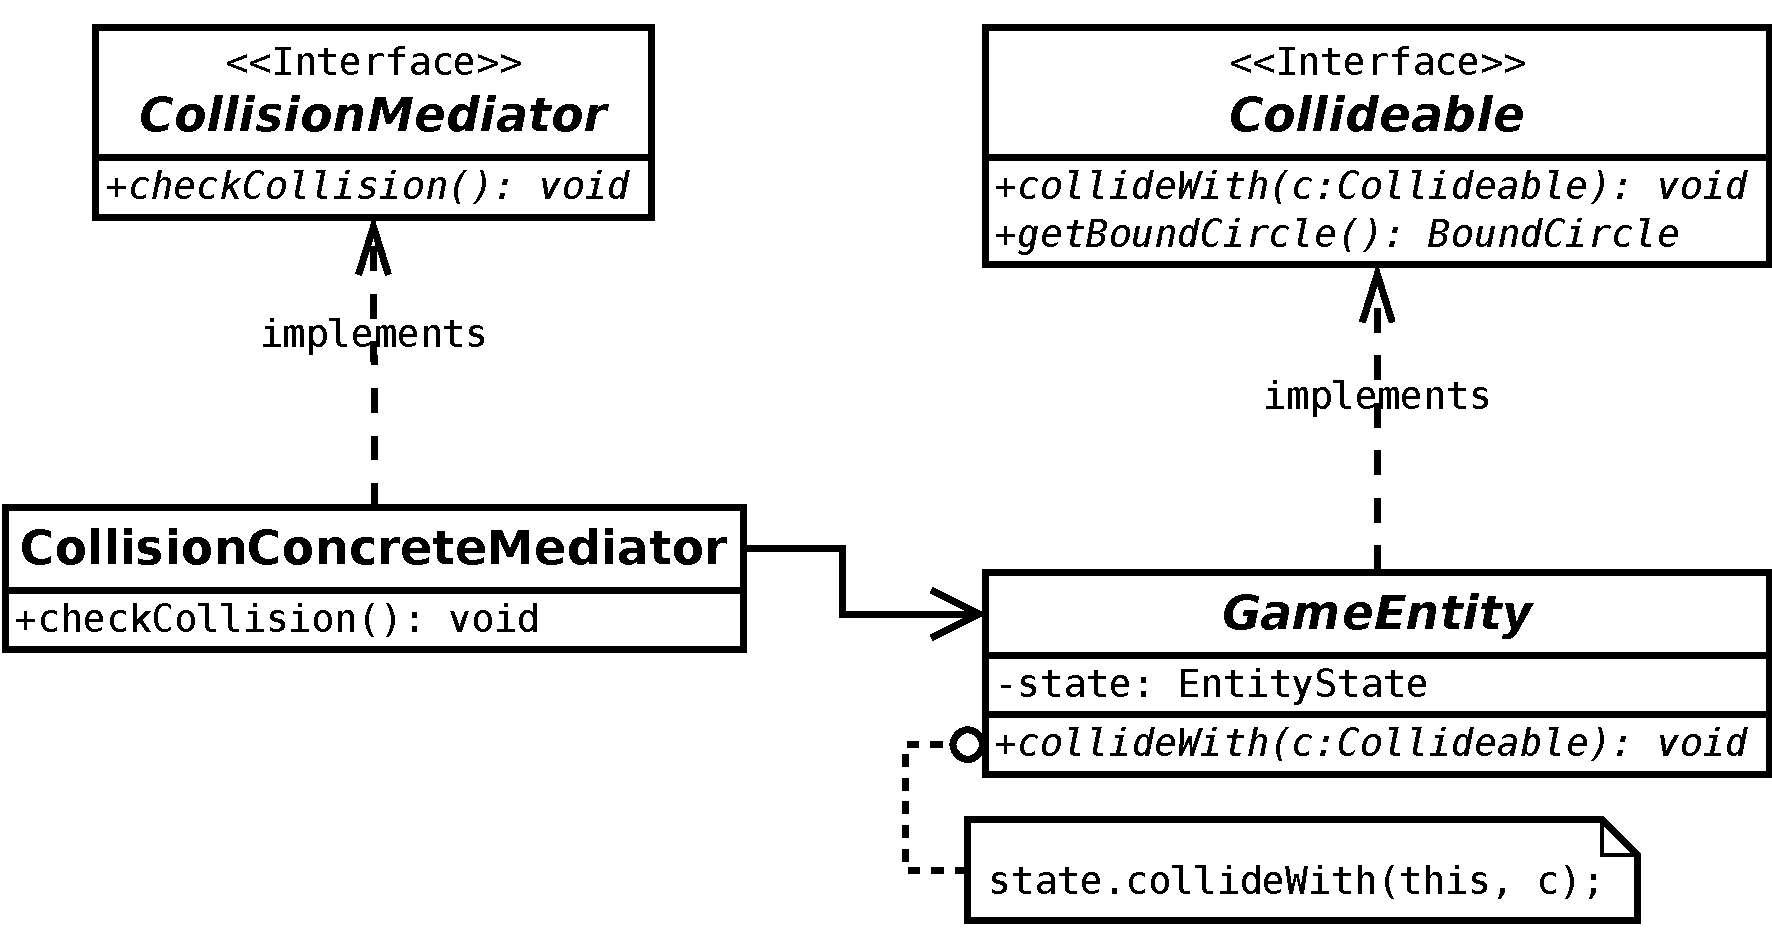
\includegraphics[width=12cm]{Mediator.pdf}
\caption{Diagramma UML del pattern \emph{Mediator}}
\label{img:Mediator}
\end{figure}


\section{Gestione del rendering grafico}
\label{sec:graphics}

Una volta definita la componente \emph{Model} del nostro sistema \emph{Model-View-Controller}, passiamo a definire la parte \emph{View}.

Generalmente i videogiochi permettono di essere visualizzati mostrando una serie di primitive grafiche per ogni entit\`a in gioco. Abbiamo dunque modellato le primitive grafiche nel modo seguente:

\begin{itemize}
\item Un'interfaccia \textsf{GraphicEntity} che rappresenta una generica primitiva grafica.
\begin{itemize}
\item La classe \textsf{GraphicSprite} che implementa \textsf{GraphicEntity} e permette di creare una \emph{sprite} indicando il nome del file da disegnare,
\item La classe \textsf{GraphicVector} che implementa \textsf{GraphicEntity} e permette di creare un vettore grafico, indicando le coordinate di inizio, di fine e il colore.
\end{itemize}
\end{itemize}

La gerarchia di classi delle primitive grafiche \`e mostrata in figura \ref{img:GraphicEntity}.

\begin{figure}[h]
\centering
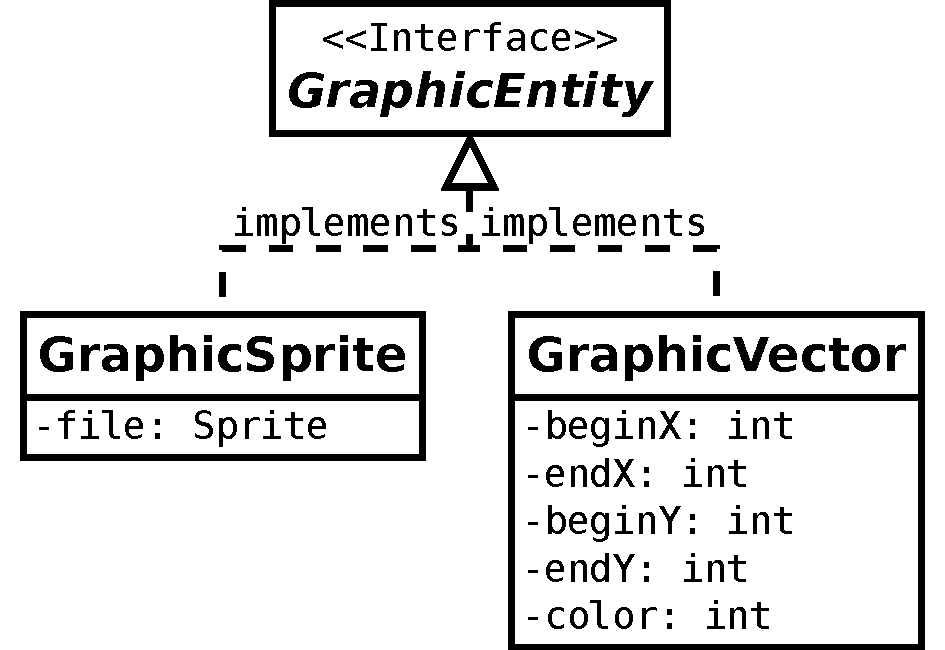
\includegraphics[width=8cm]{GraphicEntity.pdf}
\caption{Diagramma UML delle primitive grafiche}
\label{img:GraphicEntity}
\end{figure}

Abbiamo successivamente realizzato l'interfaccia \textsf{Drawable} (immagine \ref{img:Drawable}), che deve essere implementata dai soggetti che desiderano essere disegnati a scherma. L'interfaccia prevede un metodo \textsf{draw} con  un parametro di tipo \textsf{GraphicEnvironment} (il contesto grafico), si realizzano quindi tutte le operazioni necessarie a mostrare su schermo l'oggetto.

Nel nostro caso abbiamo deciso di far implementare l'interfaccia \textsf{Drawable} alla classe \textsf{GameEntity} e di lasciare l'onere di dover fornire le primitive grafiche ad ogni singolo stato sottoclasse di \textsf{EntityState}: ogni stato fornisce il metodo \textsf{getGraphicEntities} che ritorna una lista di primitive grafiche (\textsf{List}$<$\textsf{GraphicEntity}$>$) che permettono di renderizzare la singola entit\`a.

Chiariamo meglio questo concetto con un esempio: una \textsf{PowerBar} che non \`e stata mai colpita\footnote{La \textsf{PowerBar} si trova dunque nello stato \textsf{PowerBarNoHitState}} invocher\`a il metodo \textsf{getGraphicEntities} sul suo stato, ottenendo una lista di \textsf{GraphicEntity}, in particolare un solo \textsf{GraphicVector} che permette di disegnare l'oggetto \textsf{PowerBar}. Nel momento in cui avviene una collisione con un \textsf{Missile} l'oggetto \textsf{PowerBar} transisce in un nuovo stato\footnote{Lo stato \textsf{PowerBarOneHitState}} ed invocando il metodo \textsf{getGraphicEntities} si otterranno le primitive grafiche per ridisegnare la \textsf{PowerBar} che \`e stata colpita.

\begin{figure}[ht]
\centering
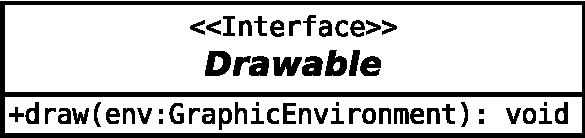
\includegraphics[width=7cm]{Drawable.pdf}
\caption{Diagramma UML dell'interfaccia \textsf{Drawable}}
\label{img:Drawable}
\end{figure}

\subsection{Uso del pattern \emph{Strategy}}

Consideriamo inoltre che dobbiamo prevedere inoltre un meccanismo per animare le primitive grafiche di una \textsf{GameEntity}, per gestire le animazioni abbiamo deciso di implementare il pattern \emph{Strategy} nei \textsf{GameEntity}.

Abbiamo realizzato la classe astratta \textsf{DrawStrategy} che contiene il metodo \textsf{drawEntity}: questo metodo accetta due parametri, un \textsf{GraphicEnvironment} dove poter disegnare e una lista di \textsf{GraphicEntity}. Abbiamo inoltre fornito due strategie concrete:

\begin{itemize}
\item \textsf{DrawVectors} che disegna semplicemente l'elenco dei vettori forniti sull'ambiente grafico
\item \textsf{DrawSprites} che anima le sprites fornite, disegnano una delle sprites nella lista a turno.
\end{itemize}

La \textsf{DrawStrategy} iniziale viene impostata tramite il metodo astratto \textsf{createInitialStrategy} della classe \textsf{GameEntity}, utilizzando il pattern \emph{Factory Method}, in un modo analogo a quanto avviene con lo stato (sezione \ref{sec:factory}).

\`E quindi possibile cambiare strategia a runtime usando il metodo \textsf{setStrategy}, oppure realizzare strategie pi\`u complesse, che prevedano animazioni pi\`u fluide, unendo sprite e vettori assieme.

Le classi coinvolte nell'utilizzo del pattern \emph{Strategy} sono mostrate nel diagramma in figura \ref{img:Strategy}

\begin{figure}[h]
\centering
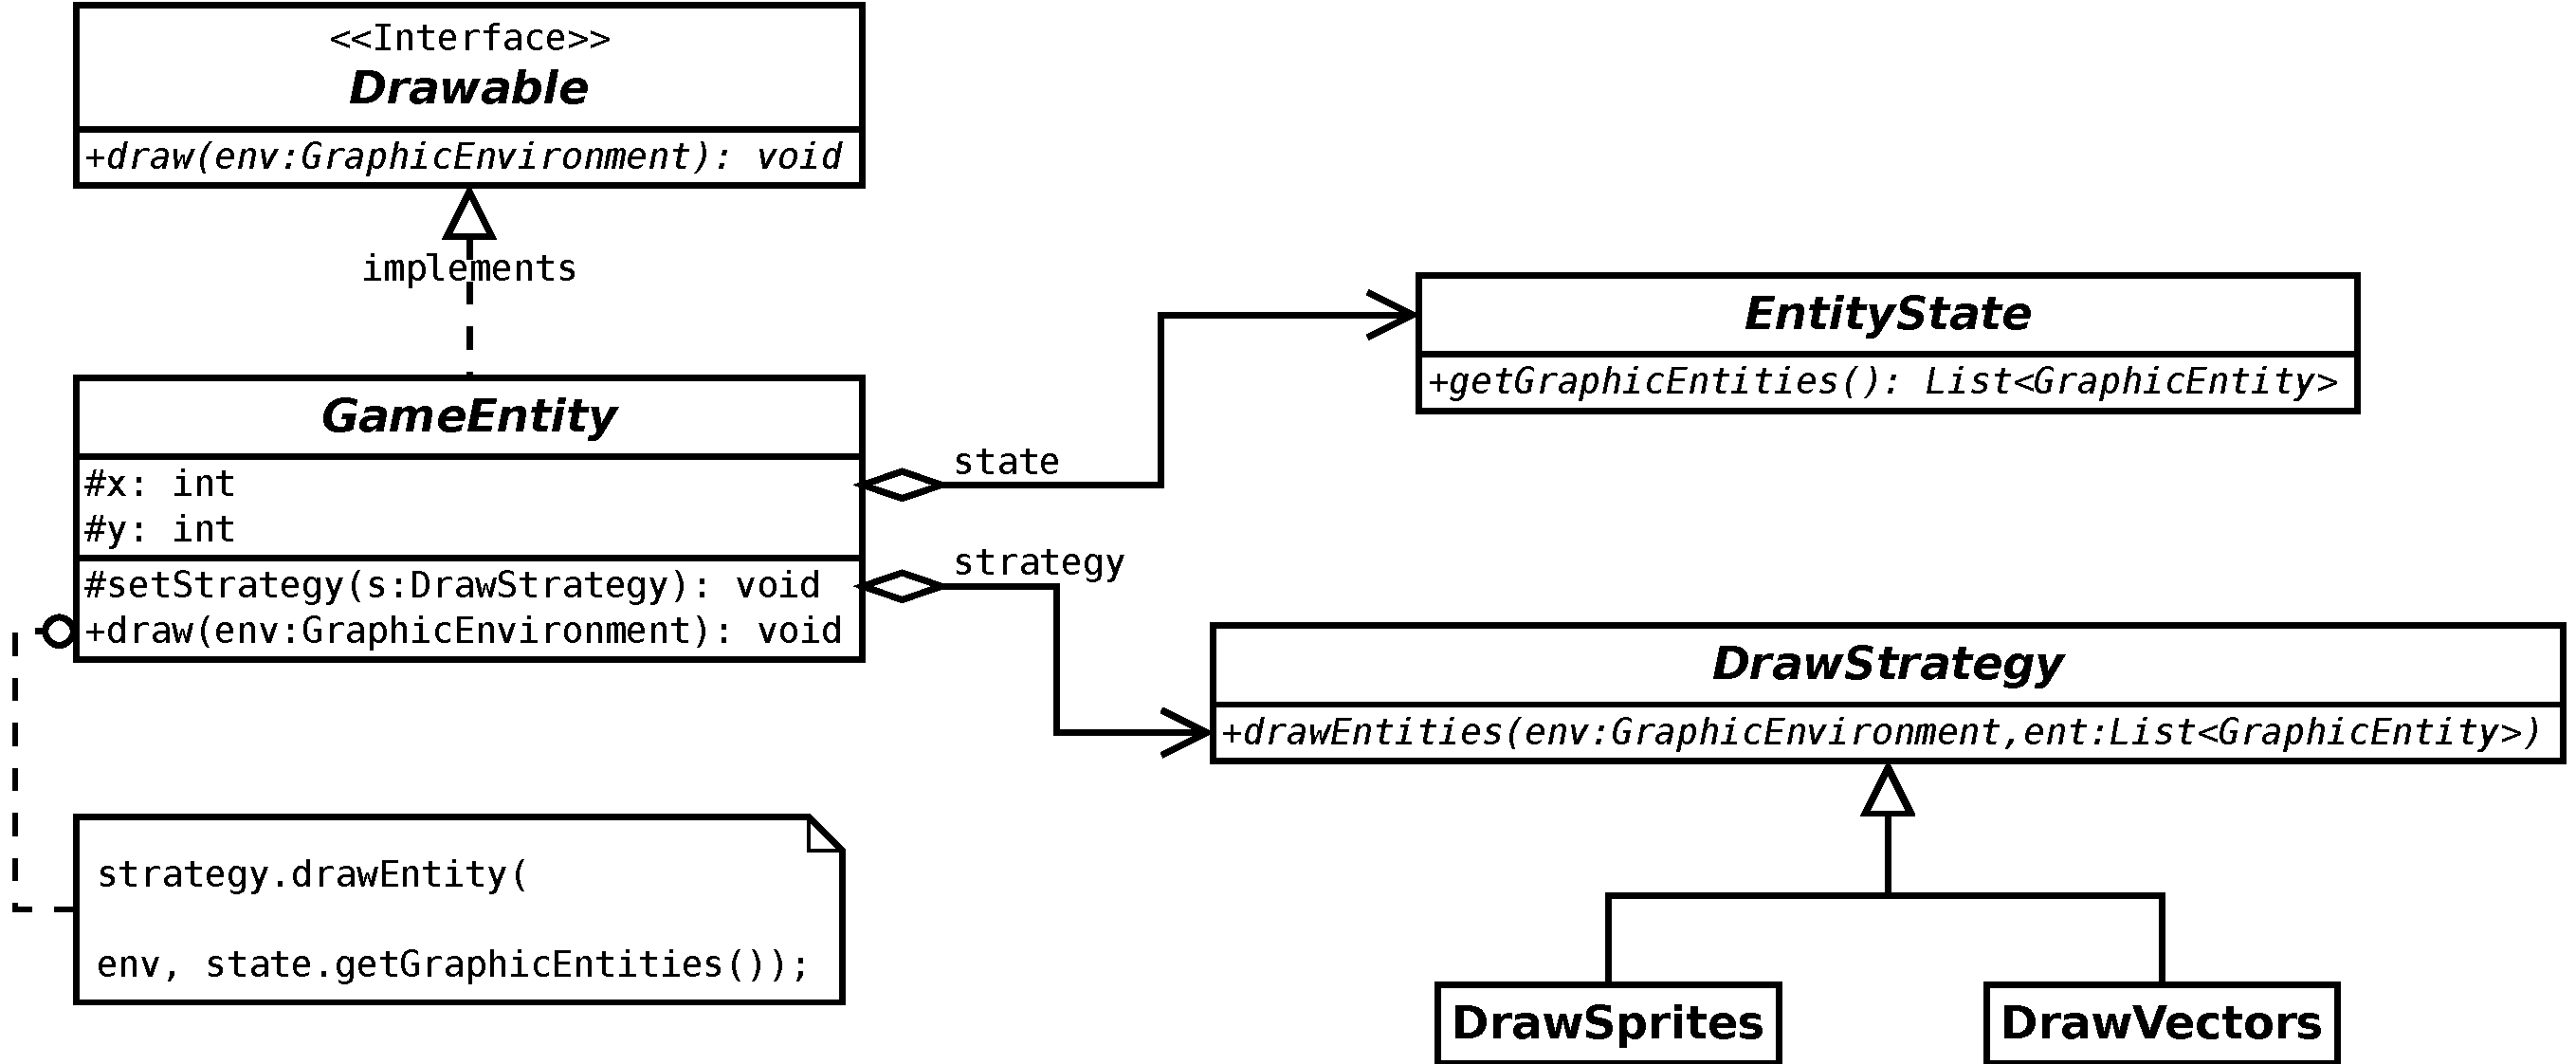
\includegraphics[width=14cm]{Strategy.pdf}
\caption{Diagramma UML del pattern \emph{Strategy}}
\label{img:Strategy}
\end{figure}

\section{Gestione dell'engine di gioco}
\label{sec:engine}

Tutte le \textsf{GameEntity} devono essere mantenute da una classe che si occuper\`a di gestire il ciclo di rendering. Questa classe \`e \textsf{GameEngine}, che mantiene i riferimenti a

\begin{itemize}
\item La lista delle \textsf{GameEntity} in gioco
\item Il \textsf{CollisionMediator}
\item I contesti grafici dove effettuare il rendering (\emph{back buffer} e \emph{display buffer})
\end{itemize}

Inoltre \textsf{GameEngine} deve offrire i metodi per
\begin{itemize}
\item Inizializzare lo stato di gioco,
\item Avviare il ciclo di gioco,
\item Interrompere il ciclo di gioco,
\item Aggiungere un'entit\`a al gioco,
\item Rimuovere un'entit\`a dal gioco,
\item Interagire con un'astronave (farla ruotare, sparare, etc\dots{}),
\item Ricevere un comando (sezione \ref{sec:comandi}).
\end{itemize}

Il ciclo di gioco \`e schematizzato nell'algoritmo seguente:
\begin{enumerate}
\item Controllo se sono nello stato di gameover,
\item Rimuovo le entit\`a che si sono distrutte (\textsf{isDestroyed}),
\item Eseguo comandi che ho ricevuto dall'utente,
\item Faccio evolvere le entit\`a in gioco (\textsf{evolveEntity}),
\item Controllo se ci sono state collisioni,
\begin{enumerate}
\item Se s\`i, notifico i soggetti coinvolti,
\end{enumerate}
\item Renderizzo sul \emph{back buffer},
\item Disegno il \emph{back buffer} su schermo.
\end{enumerate}

\subsection{Utilizzo del pattern \emph{Singleton}}

L'oggetto \textsf{GameEngine} \`e fondamentale per il funzionamento del gioco, e non vogliamo che siano presenti due istanze concrete della classe, abbiamo dunque deciso di utilizzare il pattern \emph{Singleton}.

Abbiamo un campo statico privato di tipo \textsf{GameEngine} dentro la classe stessa, che mantiene il riferimento all'istanza concreta; abbiamo reso il costruttore privato e realizzato il metodo statico \textsf{getInstance} per permettere di recuperare l'istanza di \textsf{GameEngine}.

Utilizzando questo pattern possiamo inoltre evitare di dover passare i riferimenti al \textsf{GameEngine} concreto, ma recuperarli invocato il metodo statico \textsf{GameEngine.getInstance()}.

L'implementazione del pattern \emph{Singleton} \`e rappresentata dal diagramma in figura \ref{img:Singleton}

\begin{figure}[h]
\centering
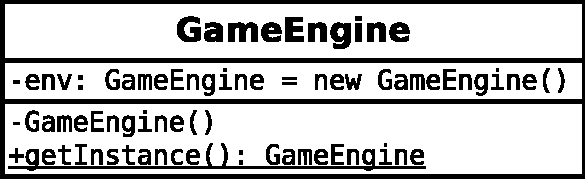
\includegraphics[width=7cm]{Singleton.pdf}
\caption{Diagramma UML del pattern \emph{Singleton}}
\label{img:Singleton}
\end{figure}

Si noti che si sta utilizzando la versione \emph{eager} del pattern \emph{Singleton} in quanto si inizializza subito l'istanza concreta, questo per evitare eventuali problemi di concorrenza; l'impatto in termini di performance \`e trascurabile.

\subsection{Utilizzo del pattern \emph{Decorator}}

Il videogioco deve prevedere anche la modalit\`a \textit{windowed}. Aggiungere la seguente modalit\`a consiste fondamentalmente in aggiungere del comportamento alla fase di rendering iniziale del videogioco.

All'avvio il gioco determina le dimensioni dell'area che pu\`o utilizzare per effettuare le operazioni di rendering grafico. Aggiungere la modalit\`a \textit{windowed} consiste in ridimensionare quest'area e aggiungere gli elementi grafici della finestra (bordi, bottoni, men\`u, etc\dots{}).

Trovandoci in una situazioni in cui si sta estendendo una funzionalit\`a, si \`e deciso di utilizzare il pattern \emph{Decorator}, il \textsf{GameEngine} rappresenta la nostra classe base, la classe astratta \textsf{GameDisplay} rappresenta la radice della gerarchia che definisce le operazioni comuni a \textsf{GameEngine} e ai decorator.

Abbiamo inoltre realizzato la classe \textsf{WindowDecorator} che rappresenta l'unico \textit{decorator} concreto, abbiamo omesso la classe astratta padre della gerarchia dei \emph{decorator} in quanto non vi erano altri \emph{decorator} concreti.

\textsf{WindowDecorator} mantiene un riferimento \textsf{component} a un oggetto di tipo \textsf{GameDisplay} (nella fattispecie il \textsf{GameEngine}), di cui estende il comportamento. In particolare il metodo \textsf{renderWindow} esegue dapprima lo stesso metodo su \textsf{component} ed aggiunge la logica della finestra.

Le classi coinvolte nell'implementazione del pattern \emph{Decorator} sono raffigurate nel diagramma in figura \ref{img:Decorator}.

\begin{figure}[h]
\centering
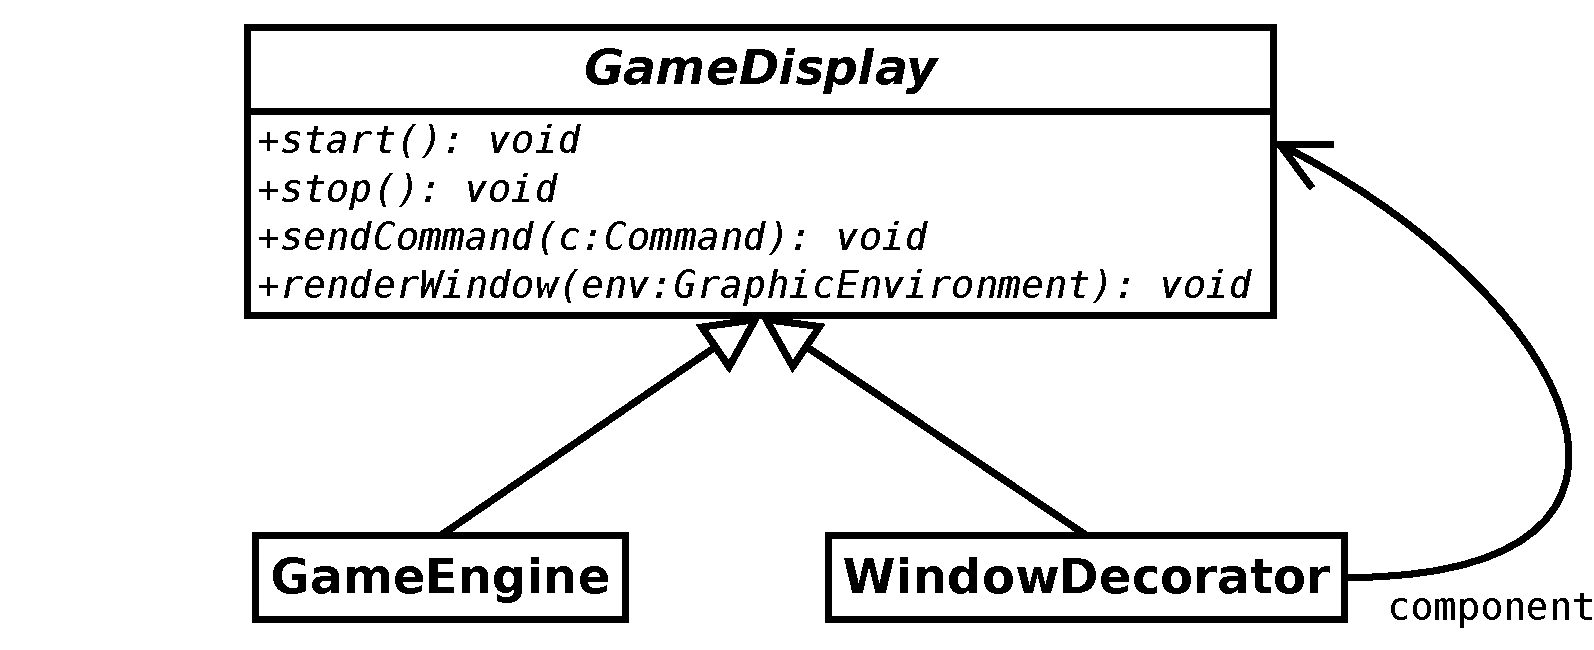
\includegraphics[width=12cm]{Decorator.pdf}
\caption{Diagramma UML del pattern \emph{Decorator}}
\label{img:Decorator}
\end{figure}

\section{Gestione dei comandi}
\label{sec:comandi}

La gestione dei comandi rappresenta il componente \emph{Controller} del sistema \emph{Model-View-Controller}. \`E bene definire quale sar\`a il flusso che dovr\`a percorrere l'input utente al fine di arrivare al modello e poterlo mutare.

Si \`e deciso in particolare di utilizzare i pattern \emph{Command} e \emph{Chain of responsability} per modellare la gestione dei comandi.

\subsection{Utilizzo del pattern \emph{Command}}

La prima classe che presentiamo \`e la classe \textsf{KeyEventManager}, che implementa l'interfaccia \textsf{java.swing.event.KeyListner}\footnote{\`E stata implementata questa interfaccia in modo da poter utilizzare facilmente l'oggetto con il framework Java Swing}, \`e si occupa di raccogliere gli eventi da tastiera dell'utente e li trasforma in comandi.

I comandi vengono modellati dalle classi che implementano l'interfaccia \textsf{Command}: \textsf{CommandRotate}, \textsf{CommandFire} e \textsf{CommandPropel} che rappresentano gli omonimi comandi da realizzare sull'astronave.

La classe che si occupa della gestione dei comandi \`e \textsf{GameEngine} che mantiene una lista di comandi da eseguire e si occupa di eseguirli ad ogni ciclo di rendering. Si \`e deciso di gestire i comandi in questo modo per non far interferire la frequenza di arrivo dei comandi con la frequenza di esecuzione del ciclo di rendering.

La classe \textsf{GameEngine} svolge il ruolo sia di \emph{Invoker}, in quanto \`e lei che invoca il metodo \textsf{execute} sui comandi, sia il ruolo di \emph{Receiver}, in quanto i comandi eseguono metodi di \textsf{GameEngine} per far evolvere lo stato (\textsf{rotateSpaceShip}, etc\dots{}).

La classe \textsf{KeyEventManager} svolge invece il ruolo di \emph{Client} del pattern, esso crea una volta singola tutti i comandi (al fine di guadagnarne in performance) e li recapita all'\emph{Invoker} appena riceve un input.

Le classi coinvolte nell'implementazione del pattern \emph{Command} sono raffigurate nel diagramma in figura \ref{img:Command}.

\begin{figure}[h]
\centering
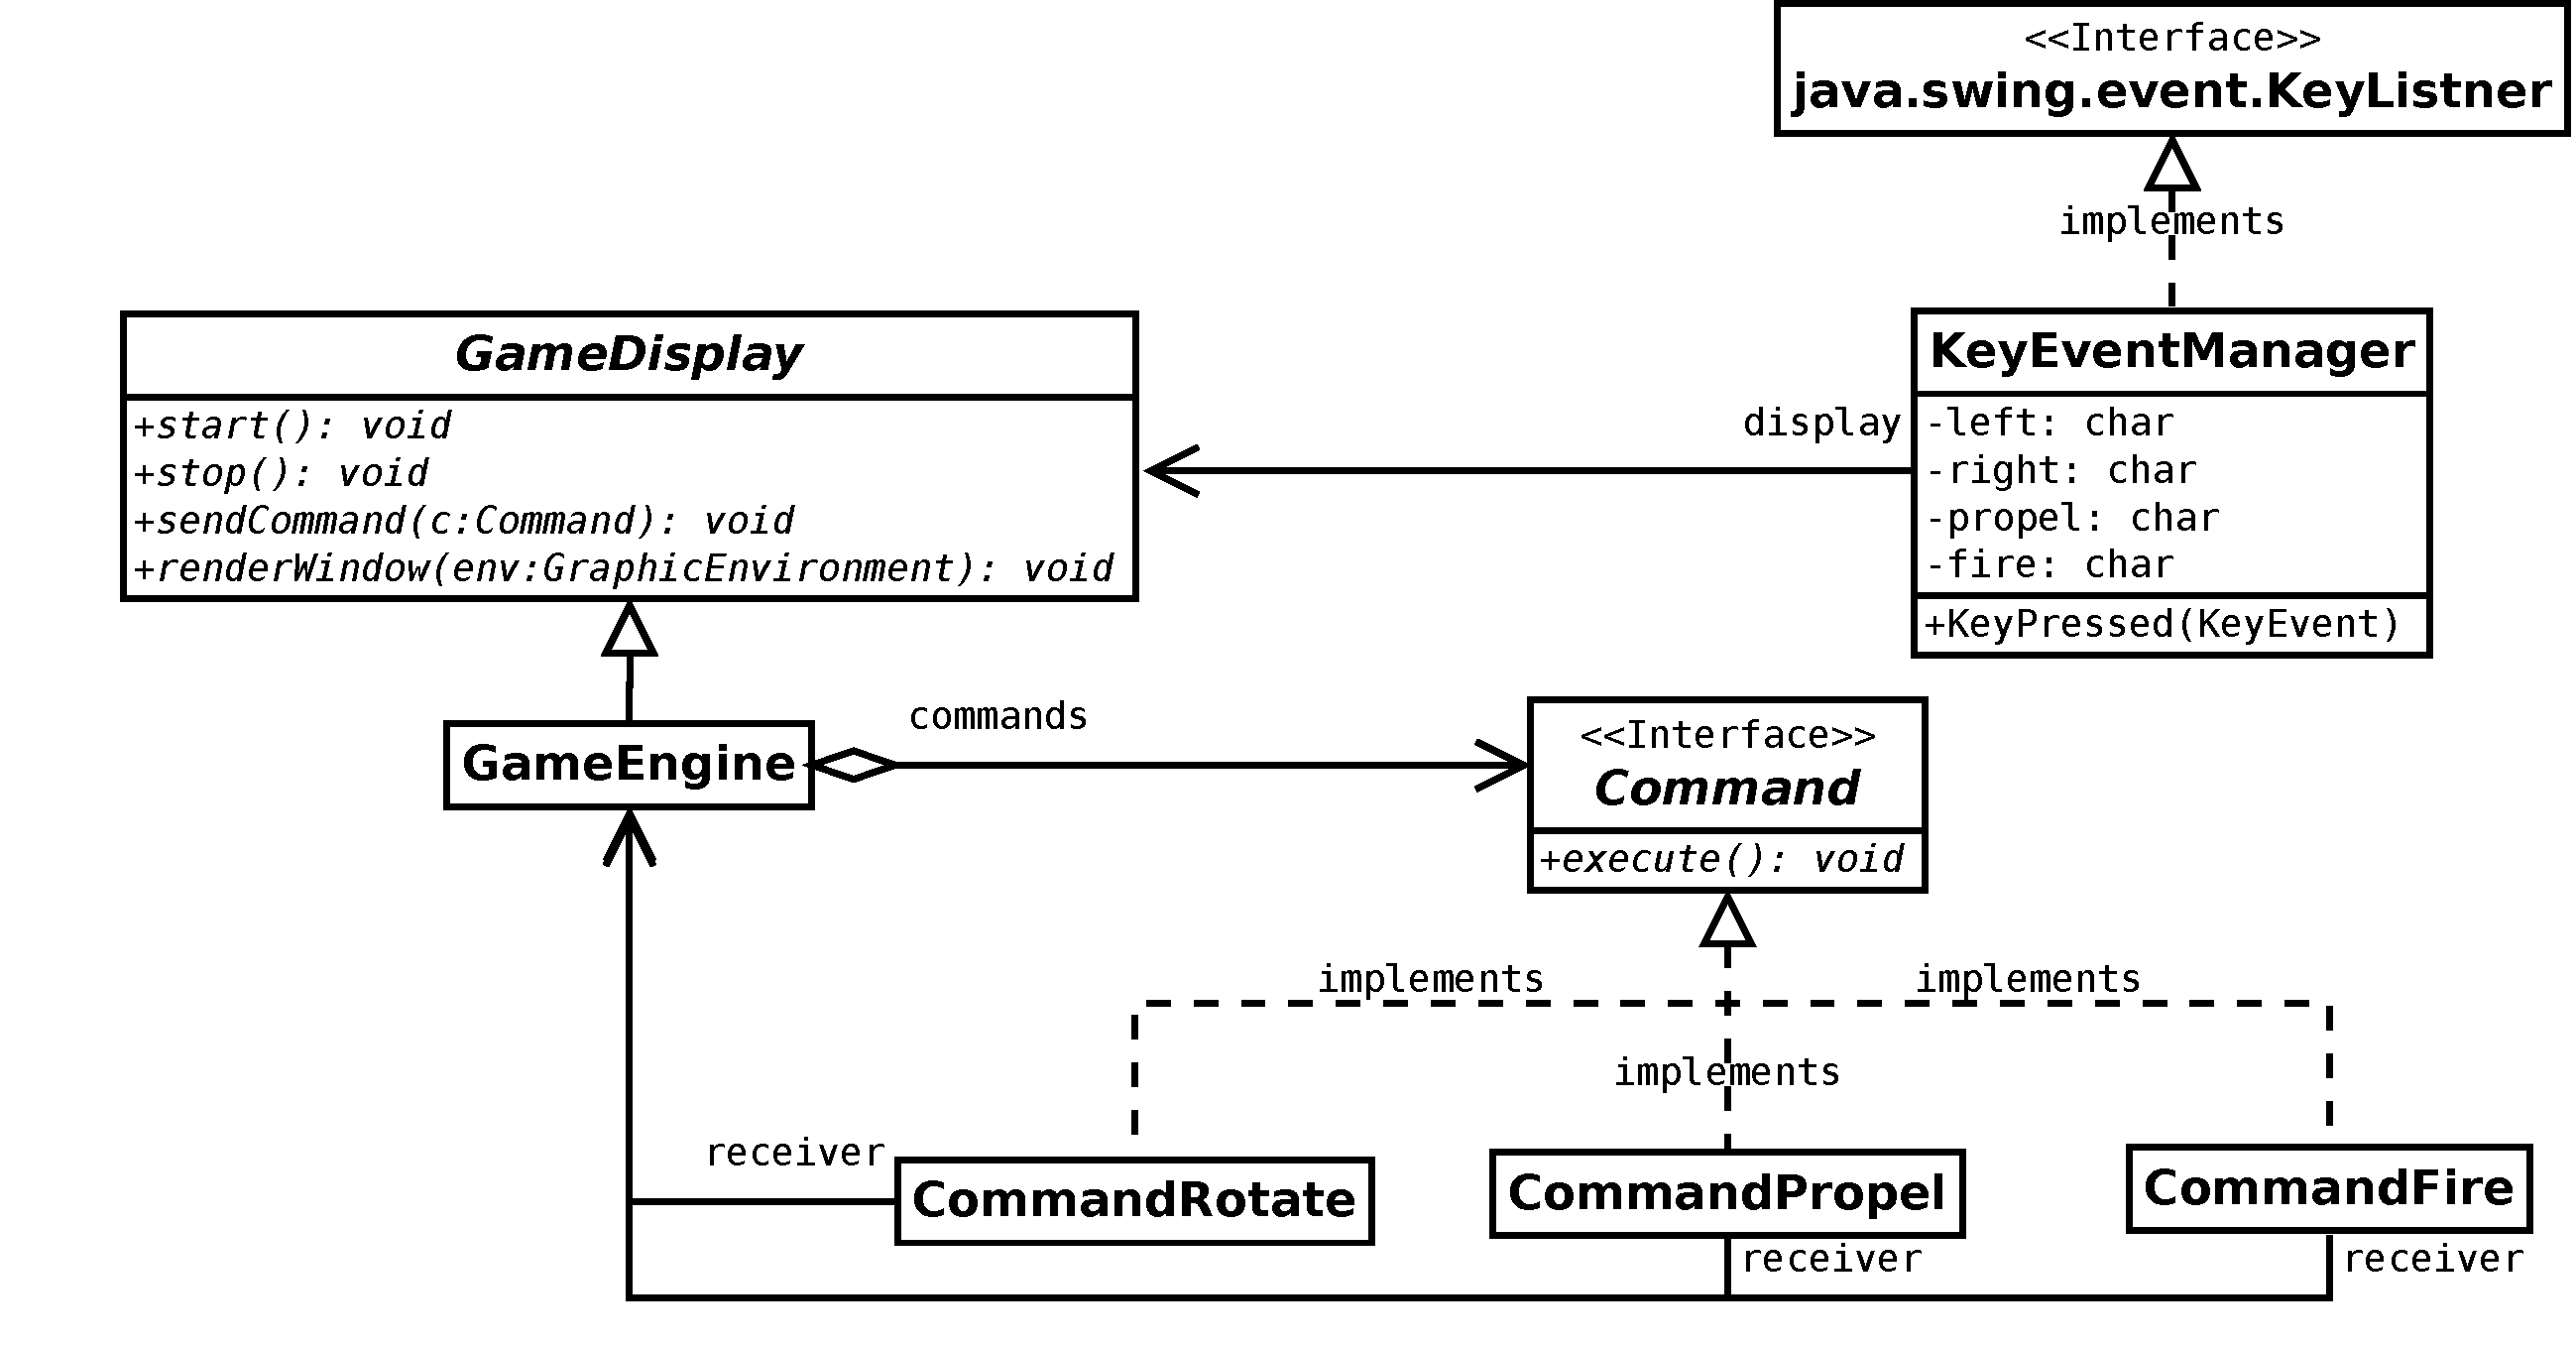
\includegraphics[width=15cm]{Command.pdf}
\caption{Diagramma UML del pattern \emph{Command}}
\label{img:Command}
\end{figure}

\subsection{Utilizzo del pattern \emph{Chain of reponsability}}

Si \`e deciso di utilizzare la struttura realizzata con il pattern \emph{Decorator} per implementare il pattern \emph{Chain of reponsability}: aggiungendo il metodo \textsf{receiveCommand} a \textsf{GameDisplay} prevediamo che ogni oggetto della gerarchia dei \textit{decorator} abbia questo metodo.

Quando il \textsf{KeyEventManager} invier\`a un comando al \textsf{GameDisplay}, il \textit{decorator} pi\`u esterno\footnote{Nel nostro caso abbiamo solamente un \emph{decorator} concreto (\textsf{WindowDecorator}), ma nulla vieta di poter scrivere altri \textit{decorator}} potr\`a decidere se gestire il comando e non propagarlo ulteriormente, oppure passare il comando al proprio \textsf{component} invocando il solito comando \textsf{receiveCommand}.

Si noti come, malgaro le classi siano le stesse, il flusso di esecuzione \`e invertito: nel caso del metodo \textsf{renderWindow}, il decorator pi\`u esterno chiedere prima l'esecuzione al \textsf{component} ed estende successivamente con il proprio comportamento; nel caso del metodo \textsf{receiveCommand} si esegue prima la logica del \textit{decorator} verificando se \`e possibile gestire il comando, e successivamente lo si propaga al \textsf{component}.

Le classi coinvolte sono le stesse del diagramma in figura \ref{img:Decorator}.

\section{Avvio e terminazione del gioco}
\label{sec:avvio}

Tutte queste classi che sono state presentate devono essere istanziate correttamente e nel giusto ordine. Questo potrebbe creare problemi per l'utilizzatore delle classi, si \`e quindi pensato di realizzare un classe unica che si occupi di creare gli oggetti necessaria e che esponga i metodi necessari ad eseguire le operazioni basilari del videogioco.

Questa classe \`e la classe \textsf{GameFacade}, che utilizza il pattern \emph{Façade}.

\subsection{Utilizzo del pattern \emph{Façade}}

\begin{figure}[h]
\centering
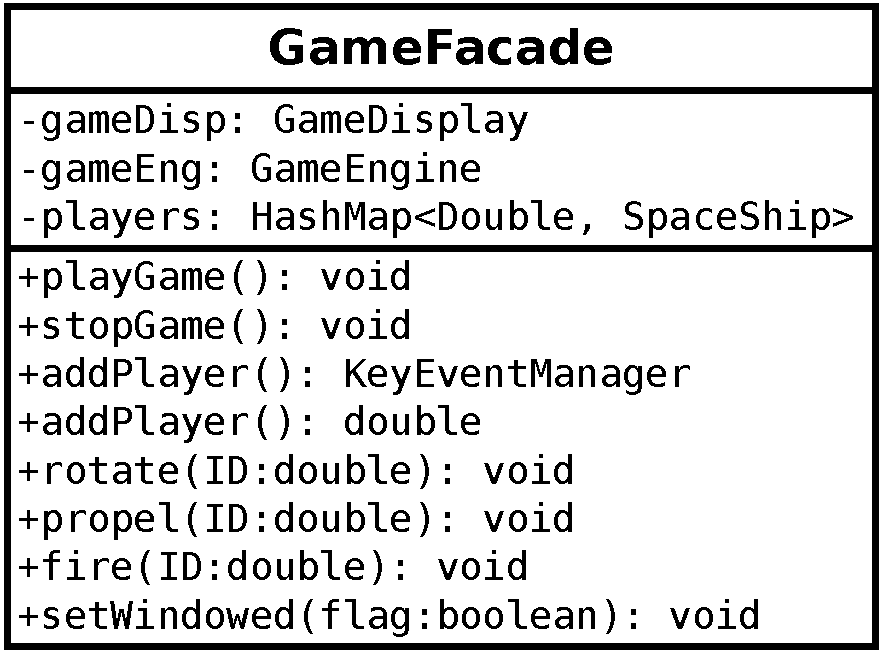
\includegraphics[width=7cm]{Facade.pdf}
\caption{Diagramma UML del pattern \emph{Façade}}
\label{img:Facade}
\end{figure}

La classe \textsf{GameFacade} (mostrata nel diagramma in figura \ref{img:Facade}) mantiene il riferimento al \textsf{GameDisplay} e al \textsf{GameEngine} costruendo l'eventuale \textsf{WindowDecorator}.

La classe mantiene inoltre l'elenco dei giocatori in una \textsf{HashMap}$<$\textsf{Double}, \textsf{SpaceShip}$>$, associando un ID ad ogni astronave creata, tale ID servir\`a per associare il giocatore reale alla propria astronave.

I metodi che offre sono:
\begin{itemize}
\item \textsf{playGame} e \textsf{stopGame} per avviare/terminare il videogioco.
\item \textsf{addPlayer(): KeyEventManager} che crea un nuovo giocatore, e ritorna un nuovo \textsf{KeyEventManager}, utilizzabile all'interno di una finestra Java Swing.
\item \textsf{addPlayer(): double} che crea un nuovo giocatore, ma ritorna invece l'ID dell'astronave appena generata.
\item \textsf{rotate}, \textsf{propel} e \textsf{fire}, che permettono di interagire con l'astronave, necessitano dell'ID dell'astronave che si vuole comandare.
\item \textsf{setWindowed} per togliere/aggiungere il \textsf{WindowDecorator} a runtime.
\end{itemize}

Chiaramente un utente pu\`o decidere di usare la versione di \textsf{addPlayer} che ritorna un \textsf{KeyEventManager}, collegarlo ad un componente Swing e non preoccuparsi pi\`u della gestione dell'input, oppure utilizzare la versione che ritorna l'ID, e gestire l'input in modo da invocare i comandi.

Un esempio di utilizzo del primo meccanismo \`e mostrato nella classe di esempio \textsf{SimpleClient}.

\section{Gestione del multiplayer}
\label{sec:multiplayer}

Una progettazione modulare come quella realizzata affidandosi ai \emph{design patterns} pu\`o aiutarci facilmente in fase di ampliamento. Si pensi ad esempio al caso in cui si voglia permettere ad un secondo giocatore di interagire in remoto.

Per permettere il gioco remoto si \`e deciso di utilizzare il pattern \emph{Remote Proxy} unitamente alla tecnologia Java RMI (\emph{Remote Method Invocation}).

\subsection{Utilizzo del pattern \emph{Remote Proxy}}

\`E stata dappirma definita l'interfaccia \textsf{RemoteGame} (che estende l'interfaccia \textsf{java.rmi.Remote}) in modo da definire i metodi invocabili da un client.

Dopodich\'e si \`e dichiarata la classe  \textsf{GameFacade} come sottoclasse della classe  \textsf{java.rmi.server.UnicastRemoteObject} e si \`e implementata le precedente interfaccia
\textsf{RemoteGame}.

\`E dunque possibile esporre un oggetto \textsf{GameFacade} tramite il protocollo RMI in modo che possa essere raggiungibile da parte di un altro \emph{host} nella rete. L'host remoto potr\`a recuperare un oggetto di tipo \textsf{RemoteGame} su cui potr\`a invocare i metodi previsti dall'interfaccia.

L'interfaccia \textsf{RemoteGame} prevede sostanzialmente gli stessi metodi di \textsf{GameFacade}, apparte per il metodo \textsf{addPlayer(): KeyEventManager} in quanto \textsf{KeyEventManager} non \`e un oggetto \textsf{Serializable} e non pu\`o essere trasmesso sulla rete: ci\`o comporta che un utente remoto sia obbligato ad utilizzare il proprio ID ed ad invocare sull'oggetto \textsf{RemoteGame} i metodi \textsf{rotate}, \textsf{propel} e \textsf{fire}.

Sono state realizzate le classi \textsf{RemoteClient} e \textsf{RemoteServer} che realizzano rispettivamente il client e il server di gioco, e che necessitano dei parametri di rete per funzionare (host e porta).

Le classi coinvolte nel pattern \emph{Remote Proxy} sono mostrate nell'immagine \ref{img:Proxy}.

\begin{figure}[ht]
\centering
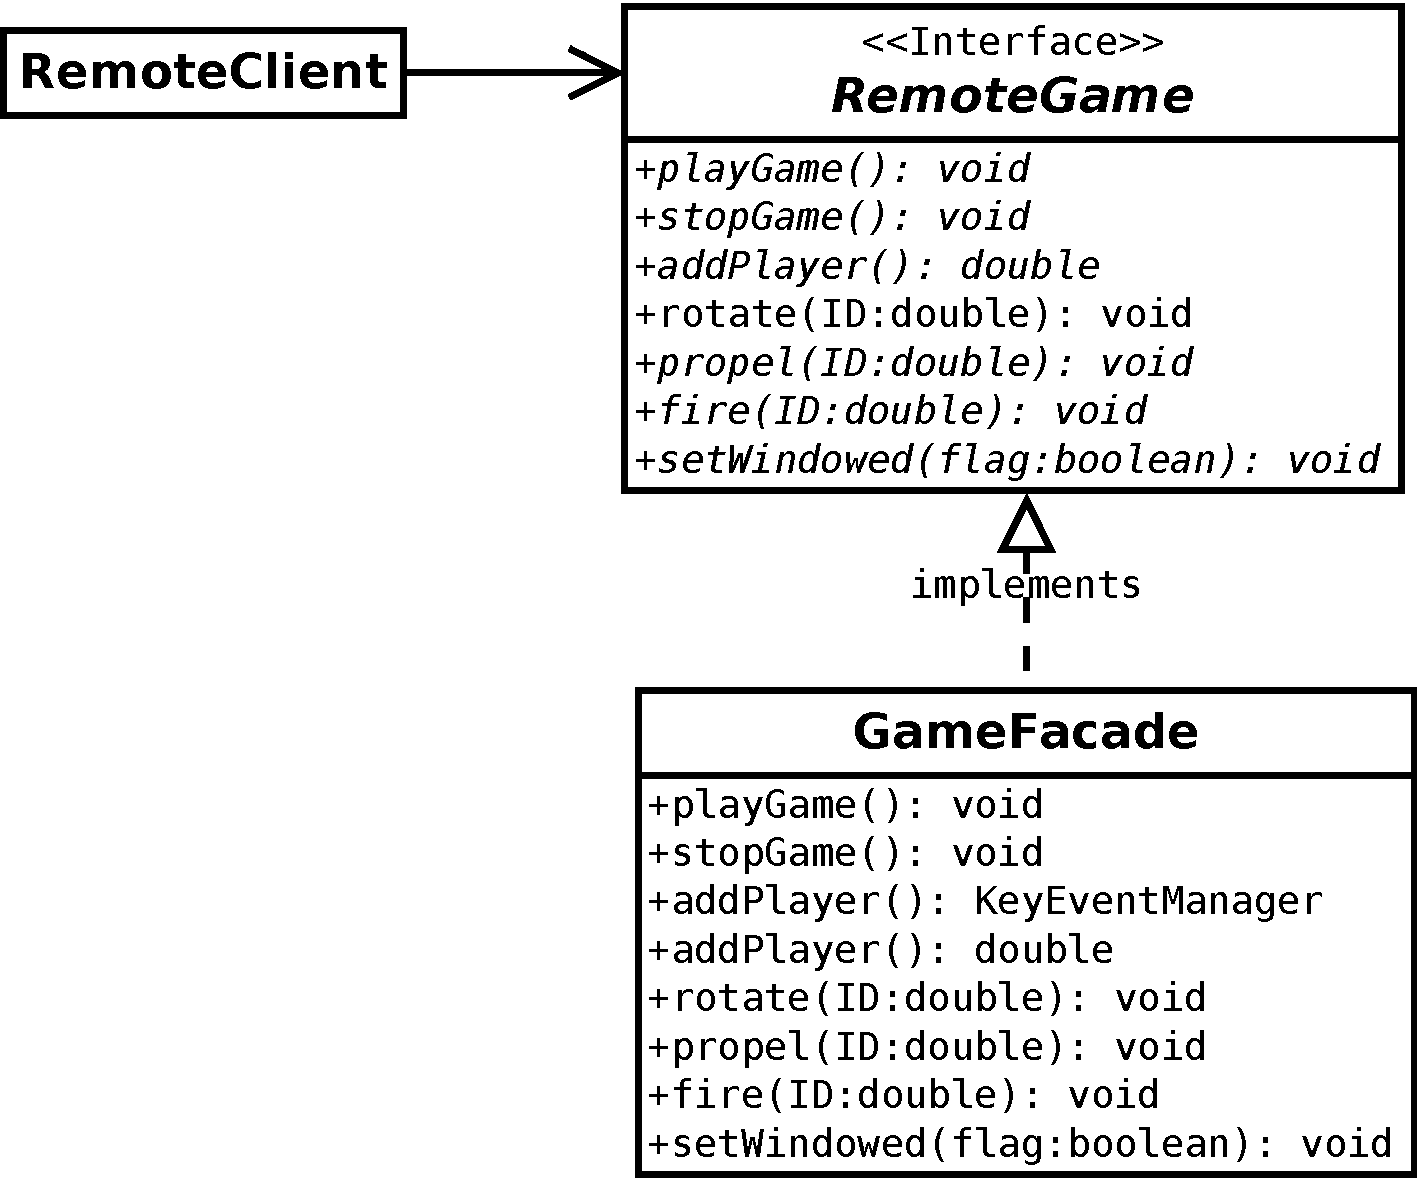
\includegraphics[width=10cm]{Proxy.pdf}
\caption{Diagramma UML del pattern \emph{Remote Proxy}}
\label{img:Proxy}
\end{figure}

\section{Descrizione dei packages}

Il software \`e stato realizzato in Java e organizzato in package di cui diamo una breve discrezione:
\begin{center}
\begin{tabular}{|l|l|}
\hline
\textbf{Nome package} & \textbf{Descrizione} \\
\hline
\textsf{it.ncorti.tdp.core} & \pbox{9cm}{Contiene le classi che costituiscono il core del gioco, in particolare \textsf{GameEngine}} \\
\hline
\textsf{it.ncorti.tdp.core.entities} & \pbox{9cm}{Contiene le classi che costituiscono le possibili entit\`a presenti nel gioco, e le classi relative al meccanismo di gestione delle collisioni} \\
\hline
\textsf{it.ncorti.tdp.graphics} & \pbox{9cm}{Contiene le classi che contengono i meccanismi per realizzare il rendering grafico del gioco} \\
\hline
\textsf{it.ncorti.tdp.user} & \pbox{9cm}{Contiene le classi che gestiscono gli eventi di input utente} \\
\hline
\textsf{it.ncorti.tdp.user.rmi} & \pbox{9cm}{Contiene le classi che permettono il gioco da remoto} \\
\hline
\end{tabular}
\end{center}


\section{User guide}
\label{sec:guide}

Il software \`e stata corredato di un file \textbf{ant} (il file \texttt{build.xml}) che offre dei target per automatizzare il processo di compilazione e di esecuzione del software.

Per compilare il software \`e necessario posizionarsi all'interno della directory dove \`e contenuto il software ed invocare da terminale il comando

\begin{lstlisting}[basicstyle=\ttfamily]
ant build
\end{lstlisting}

che provveder\`a ad invocare il compilatore \texttt{javac} per compilare i sorgenti presenti all'interno della cartella \texttt{src/}, i file \texttt{.class} generati si troveranno all'interno della cartella \texttt{bin/}. 

Per pulire la cartella \texttt{bin/} al fine di avere un ambiente pulito per poter effettuare una nuova compilazione \`e possibile utilizzare il target
\begin{lstlisting}[basicstyle=\ttfamily]
ant clean
\end{lstlisting}

\`E infine possibile generare un file \texttt{jar} contenente tutti i file compilati e tutte le librerie necessarie all'esecuzione. Per farlo \`e sufficiente invocare il target
\begin{lstlisting}[basicstyle=\ttfamily]
ant jar
\end{lstlisting}
Verr\`a generato un file chiamato \texttt{starcastle.jar} all'interno della cartella principale del software.
Per avviare il file \texttt{jar} \`e necessario invocare il comando
\begin{lstlisting}[basicstyle=\ttfamily]
java -jar starcastle.jar <char-left> <char-right> <char-propel> <char-fire>
\end{lstlisting}

Dove $<$\texttt{char-left}$>$ e seguenti rappresentano i caratteri da utilizzare per i tasti sinistra, destra, accelera e spara.

\subsection{Documentazione}

Al fine di rendere il codice sorgente pi\`u comprensibile, il software \`e stato corredato di documentazione. In particolare tutte le parti del codice sorgente che potrebbero risultare di difficile comprensione sono state commentate. Inoltre ogni funzione e classe del software \`e stata documentata con il formato \textsf {javadoc}, la documentazione generata pu\`o essere visionata all'interno della cartella \textsf{doc/} e pu\`o essere rigenerata utilizzando il comando
\begin{lstlisting}[basicstyle=\ttfamily]
ant javadoc
\end{lstlisting}

La documentazione in javadoc pu\`o essere visionata anche online al link seguente \url{http://cortinico.github.io/tdp/}.

Per una comprensione organica del software si consiglia la lettura della seguente relazione nella sua interezza. La presente relazione viene rilasciata in Pdf ed in \LaTeX\ e pu\`o essere visionata all'interno della cartella \texttt{doc/tex/}.

\subsection{Avvio della software locale}

Una volta compilato il software \`e possibile testarlo in locale utilizzando il comando
\begin{lstlisting}[basicstyle=\ttfamily]
ant Simple [-Dleft=<char> -Dright=<char> -Dpropel=<char> -Dfire=<char>]
\end{lstlisting}

Con le opzioni \texttt{-Dleft=} e seguenti \`e possibile impostare la mappatura dei tasti per il gioco. Se non vengono fornite verr\`a utilizzata la configurazione \textsf{w a s d}.

Verr\`a mostrata una piccola finestra Swing (vedi immagine \ref{img:Swing}) che permetter\`a di catturare gli eventi di tasti premuto e farli elaborare al gioco.

\subsection{Avvio della software remoto}

Per avviare il server remoto \`e possibile utilizzare il target
\begin{lstlisting}[basicstyle=\ttfamily]
ant Server [-Dhost=<hostname>] [-Dport=<port>]
\end{lstlisting}

Con le opzioni \texttt{-Dhost=} e \texttt{-Dport=} seguenti \`e possibile impostare il proprio hostname/indirizzo IP e la porta di ascolto. Se non forniti il server si mette in ascolto come localhost (127.0.0.1) sulla porta (34567), assicurarsi che la porta indicata non sia occupata e che non vi siano problemi nella configurazione di rete.

Per avviare il client \`e invece sufficiente invocare il comando 
\begin{lstlisting}[basicstyle=\ttfamily]
ant Client [-Dleft=<char> -Dright=<char> -Dpropel=<char> -Dfire=<char>] [-Dhost=<hostname>] [-Dport=<port>]
\end{lstlisting}

Le opzioni hanno significati uguali a quelle gi\`a presentate.

\newpage
\listoffigures

\end{document}
